\documentclass[a4paper, 12pt]{article}
%%%%%%%%%%% Pacotes utilizados
\usepackage[brazil]{babel}
\usepackage[utf8]{inputenc}
\usepackage{verbatim}
\usepackage[normalem]{ulem} %para 
\usepackage{indentfirst}
\usepackage{setspace}
\usepackage{float}
\usepackage{graphicx}
\usepackage{svg}

%%%%%%%%%%%%%%% Configurações
\setlength{\textwidth}{16cm}
\setlength{\textheight}{23cm}
\setlength{\evensidemargin}{-1cm} \setlength{\oddsidemargin}{0.5cm}
\setlength{\topmargin}{0cm}

\usepackage{fancyhdr}

\pagestyle{fancy}
\fancyhf{}
\lhead{\textbf{Nome:} Jhonatan Guilherme de Oliveira Cunha}
\rhead{\textbf{RA:} 2135590}
\cfoot{\thepage}

\hoffset= -0.4cm
\voffset=-0.5cm

%%%%%%%%%%%%% Início do documento
\begin{document}
	
	\hspace{0.3cm}
	
	\begin{large}
		\begin{center}
			\textbf{UNIVERSIDADE TECNOLÓGICA FEDERAL DO PARANÁ}\newline
			\textbf{CAMPUS CAMPO MOURÃO}
		\end{center}
	\end{large}
	
	\vspace{0.3cm}
	
	\begin{center}
		\textbf{ATIVIDADE PRÁTICA 1 - MODELAGEM DE DADOS}
	\end{center}

	\vspace{0.3cm}
	
	\onehalfspacing
	Durante a aula síncrona da disciplina de \textbf{Banco de Dados 1} no dia 01/03/2021, foi solicitado a construção de um esquema conceitual, com objetivo de projetar uma base de dados sobre uma universidade. A modelagem do diagrama \textbf{Entidade-Relacionamento} foi ilustrada via software \textit{``Draw.io''}.
	
	Veja na Figura \ref{modeloER} o modelo conceitual (Entidade-Relacionamento) desenvolvido nesta atividade.
	
	\begin{figure}[H]
		\centering
		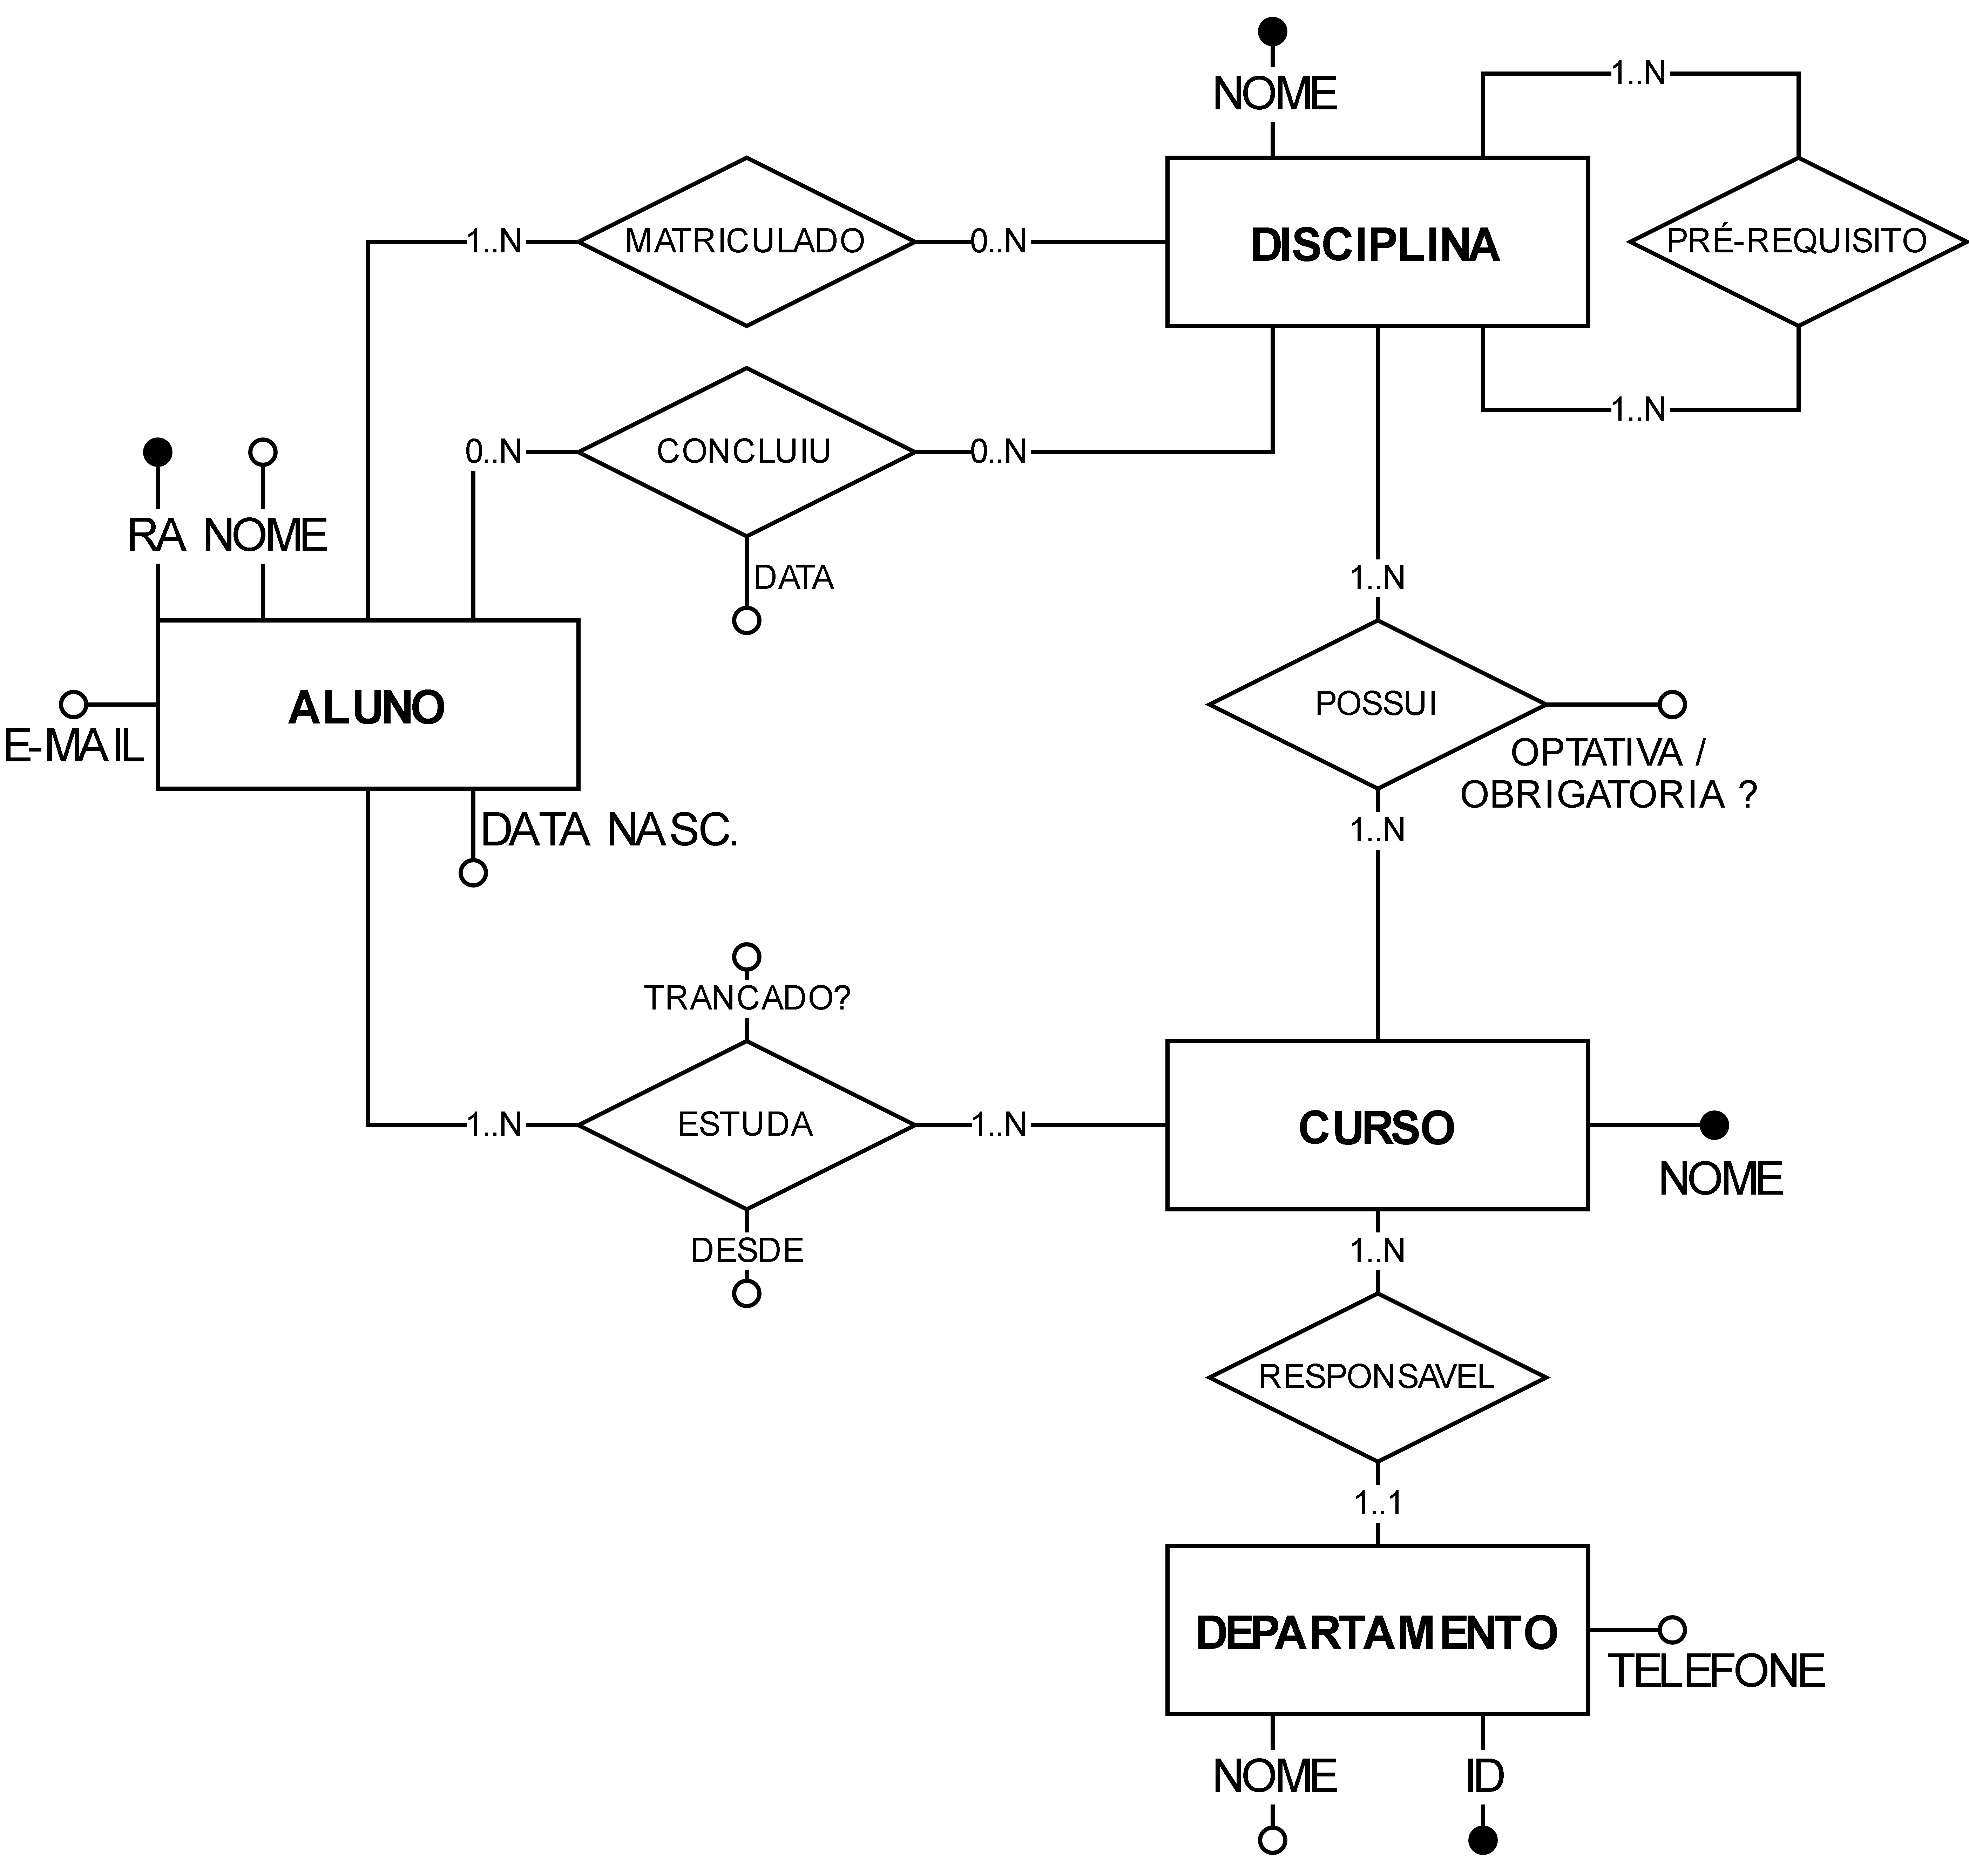
\includegraphics[scale=1.25]{resolucao.png}
				\caption{Modelo \textbf{Entidade-Relacionamento} projetado com o software \textit{Draw.io}}
		\label{modeloER}
	\end{figure}
	

\end{document}
